\documentclass[letterpaper, 11pt]{article}


%=================================================

\usepackage{fullpage, parskip}
\usepackage{fancyhdr}	%% Header and footer
\usepackage{amsmath, mathtools}
\usepackage{amssymb}	%% mathbb, \ll
\usepackage[round,authoryear]{natbib}	%% Citations
\usepackage[breaklinks,backref,bookmarks=true]{hyperref}
\usepackage{enumitem}	%% Resume numbering in enumerate
\usepackage{url}
\usepackage{graphicx}
\usepackage{tabularx}
\usepackage{subcaption}
\captionsetup{compatibility=false}
\usepackage[usenames,dvipsnames]{color}
\usepackage{pdfpages}
\usepackage{xspace}	%% Guesses whether to put space after command
\usepackage{aas_macros} %% Journal control sequences

%--------------------------------------------------
%% Header and Footer
\pagestyle{fancy}
\fancyhead{}
\renewcommand{\headrulewidth}{0.0pt}
\rfoot{Cato Sandford}
\lfoot{Summer 2012}

%%--------------------------------------------------
%% Maths macros
\def\HST{HST\xspace}
\def\psfobs{\ensuremath{{\rm PSF_{obs}}}\xspace}
\def\psfref{\ensuremath{{\rm PSF_{ref}}}\xspace}
%%--------------------------------------------------
%% Language macros
\def\etc{{\&c.}\xspace}
\def\th{\textsuperscript{th}\xspace}
\def\ra{\ensuremath{\rightarrow}\xspace}
%%--------------------------------------------------
%% Editing macros
\def\TODO#1{ {\color{red}{\bf TODO: {#1}}}\xspace}
\def\MORE{{\color{red}{\bf MORE}}\xspace}
\def\REF{{\color{OliveGreen}{\bf REF}}\xspace}
\def\FIG#1{{\bf FIGURE: }{#1}}
%%=================================================


%% Top matter
\title{Discovery Sensitivity in Human Viewable Images}
\author{Cato Sandford\thanks{Department of Physics, New York University, USA; \texttt{cato@nyu.edu}}, Phil Marshall, David Hogg}
\date{\today}

%%-------------------------------------------------

\begin{document}

\maketitle
\vspace{1cm}


\begin{abstract}
A sketch of my project with DWH and PJM: image deconvolution and colour-composition.
\end{abstract}


\begin{center}
\line(1,0){250}
\end{center}
\vspace{-0.5cm}
\tableofcontents
\vspace{-0.1cm}
\begin{center}
\line(1,0){250}
\end{center}
\newpage


%%=================================================
%% Introduction
%%=================================================

\section{Introduction}
\label{sec:intro}

For centuries, astronomers have continued to astonish the world with pictures of a Universe far richer and more magnificent than any ordinary mind could conceive. Perhaps more than any other field of science, astronomy relies on the analysis of images to draw conclusions about the natural world. Indeed, new and unusual astronomical objects, such as
galaxies, nebulae, star clusters, supernovae and so on, appear readily to
experienced viewers as they inspect new images \citep[a recent example is the amateur discovery of a quadruple star system, reported in][]{PH12}; our understanding of  the structure of, for example, galaxies can
be improved by studying their morphology, by eye\footnote{{\bf Phil:} indeed, is it not true that there is sometimes little alternative if one wants to draw meaningful conclusions about galaxy structure? Perhaps it is beyond the scope here, but it may be interesting to discuss what can be done by computers and what cannot -- the question isn't really addressed head-on even in your theory paper, yet it provides a compelling motivation for this work.} \citep[e.g.][]{Lah95, Lah++95, For++11, But11}\footnote{{\bf Phil}: We really want evidence of \emph{visual} inspection being useful, hence these references. Possibly too many.}.
Image viewing is a form of data exploration, an important step before making
quantitative measurements. But both exploration and measurement involve data
modeling, or inference: the viewer interprets the image in the context of a
model for that image that they hold.  By investigating and modeling this
viewing process, we can hope to increase the efficiency of such discoveries,
increasing the rate at which true detections are made, and reducing the
incidence of false detections. 

One way to increase the frequency with which discoveries are made  could be to
employ a larger number of experienced image viewers to look at images.  This
approach is being taken by ``citizen science'' projects such as Galaxy Zoo
(citation required\footnote{Cato, Phil: Add more zoo citations. In paper X they
found Y, in paper Z they found...}). In the Galaxy Zoo system, color composite
images of galaxies are presented to large numbers of viewers, who carry out
visual morphological studies guided by a short questionnaire. The viewers have
a wide range of experience with astronomical images, and the majority of
viewers come to the site not having viewed many astronomical images before.
The model for astrophysical objects that this group has is therefore
data-driven: their ability to spot something new depends partly on their
pre-conceived notions of what galaxies look like, but to a greater extent it
will depend on the images they have seen in the system before. Given an
inspection Zoo and a user base like this,  how should we prepare and present
the color images of galaxies, to increase the probability of an interesting
new feature being detected? This is the question we seek to answer in this
paper, taking as our archetypal interesting features the faint arcs caused by
gravitational lensing. 

Gravitational lenses enable a wide range of science projects, providing a
means to measure the mass distributions of  galaxies, groups and clusters,
independent of their luminosity or dynamical state, and giving us a rare
magnified view of the distant universe. At present almost all these projects
are limited by the small samples of lenses known, but the wide field surveys
coming online have the potential to change that. A number of optical and near
infra-red imaging surveys are planned for the next decade that together have
been predicted to contain over 10,000 new gravitational lenses, an increase in
sample size relative to the present day of around two orders of magnitude
(see, for example, \citet{O+M10}; \citet{Paw++12}\footnote{The lensing discoveries of \citet{Paw++12} arose from the dedicated visual inspection of \HST images by two astronomers. They note that for the next generation of telescope missions, the time-demands of their method will be (even more) impractical. But their work lends credence to the claim that visual inspection may yet make valuable contributions to source-discovery.}; \citet[chapter 12]{LSST09}; \citet[chapter 1, page 8]{ERB10}). Most of these
surveys will be carried out on ground-based telescopes, and will be both
multi-filter, in many cases multi-epoch, and synoptic, in order to meet a wide
range of different science requirements. The thousands of square degrees of
sky imaged, and the billions of objects catalogued, will provide a huge mine
of data to be searched for rare objects like lenses. We expect image viewing
to play a role in this search process, most likely in the form of quality
control inspection of the outputs of various automated detection algorithms.

For an image to enable discovery, it needs to be {\it informative}: that is,
it must have high quality, so that interesting features are visible to the
viewer, and it must not be confusing, so that interesting features are not
mistaken for artifacts and ignored. The quality of an astronomical image is
only partly determined by the observing conditions, telescope, and camera: the
image processing carried out in software is also important. We have additional
information about the image that we can use to improve both its resolution and
depth. The stars provide images of the imaging system point spread function
(PSF), while our understanding of the detector and the sky background provide
a model for the noise in the image: we can attempt to use both of these in
reconstructing a higher quality image. There is a significant body of
literature on this image restoration process in astronomy \citep[e.g.][]{Ric72, N+N82, S+B84, P+P93, MCS98}. We might
expect algorithms like this to be important for synoptic surveys, whose
resolution and depth varies from image to image, and from filter to filter in
a partiular field of view. Combining raw images into a color composite will
produce colored artifacts due to the mis-matched resolution in the red, green
and blue channels; while the resulting composite will have different (mean)
resolution than other elsewhere on the sky, leading to an inhomogeneity that
will hinder the development of the viewers' internal feature model as they
have to allow for the variations in image quality. However, deconvolution is
notorious for producing image artifacts if not sufficiently regularized
\citep[see, for example, comments at the end of section~1 of][]{MCS98}: such artifacts could
create more problems than the deconvolution solves, reducing the probability
of a discovery being made.  An experimental test of the sensitivity with which
an image set enables discovery is required.

In this paper we investigate a simple model-based deconvolution scheme for
resolution matching, combined with a standardised image scaling and stretch,
producing homogenized sets of color composites for inspection and then testing
their sensitivity for lensed feature detection by viewers in the Galaxy Zoo.
Using a set of $N$ realistic simulated test images for the XXX survey 
containing faint lensed features, we define a set of metrics that quantify
discovery sensitivity based on a test group of viewers responses, and 
ask the following questions:

\begin{itemize}

	\item Does simple, ``light'' deconvolution designed for making
resolution-matched composite images introduce significant colored artifacts?

	\item What target PSF-width should be used in order to
maximise discovery sensitivity in the color composite images? How does this
relate to the input images' resolution?

	\item What algorithm for choosing the color composite images' stretch and
scaling should be used, to to maximise discovery sensitivity? 

	\item Is there significant scatter in viewers' preferences regarding image
stretching and scaling, such that viewer control over these parameters is
justified?

\end{itemize}

While we focus on lensed features as our discovery targets, and the XXX
survey, we hope that our results will be of interest to the astronomical
community in general, and in particular to anyone who wants to see what they
have found in the object catalog database of a large synoptic imaging survey.

In the following two subsections, we discuss the origins of blurriness in telescope images (\ref{sec:psf}) and highlight some issues regarding the combination of band-pass data (\ref{sec:bands}). Then in section~\ref{sec:deconvolution} we outline a scheme for mitigating image bluriness. In section~\ref{sec:colour} we change tack and discuss a separate issue -- that of combining filtered images into coloured composites. These two strands are brought together in section~\ref{sec:combine}.


\subsection{The Point-Spread Function (PSF)}
\label{sec:psf}

\begin{itemize}
	\item What is it?
	\item Whence?
	\item Different in every image, sometimes varies within image	
	\item How to identify
\end{itemize}

\subsection{Bandpasses and Colour Images}
\label{sec:bands}

\begin{itemize}
	\item Photometric applications -- cheaper than spectroscopy (don't throw away photons) but yields information
	\item Build a full picture by co-adding. But from section~\ref{sec:psf} we know this can be problematic.
\end{itemize}

\newpage
%%=================================================
%% DECONVOLUTION
%%=================================================
\section{Deconvolution}
\label{sec:deconvolution}

As mentioned in the introduction, it is frequently possible and indeed desirable to reduce or control the bluriness (or PSF) of a telescope image. In this section, we describe how one might do this -- the procedure is as follows:

\begin{enumerate}
	\item Identify the astronomical sources in a FITS image.
	\item Find the point sources, and from these estimate the PSF of the image. We call this the ``observed PSF'', or \psfobs.\label{pnt:getpsf}
	\item Generate a symmetrical\footnote{Well, not actually circularly symmetric.} target PSF for the image, using the dimensions and flux properties of the image PSF of point~\ref{pnt:getpsf}. We call this the ``reference PSF'' or \psfref.\label{pnt:PSF0}
	\item Create an object which maps the observed PSF to the reference PSF. This object is called the ``kernel'' and the mapping procedure is convolution.
	\item Apply this procedure to the original image; this should correlate all the pixels in such a way as to rid the image of asymmetrical blurriness and replace it with a blurriness of known properties.
\end{enumerate}

The reader may be confused at this point as to why, if we can correctly calculate the PSF of an image, we don't simply do away with the blurriness altogether -- i.e. find a kernel which maps the PSF to a point. This would be a ``hard deconvolution'', a procedure which is compellingly discouraged by the work of \cite{MCS98} (see appendix~\ref{sec:MCS98notes} for more discussion of this paper). Following this work, we may endeavour to obtain better knowledge of the sky by reducing the PSF, but we must avoid inadvertently violating the sampling theorem, which would certainly happen if we attempted a hard deconvolution.

Once we have made the target PSF as small as possible within this restriction, we can enforce that it be symmetrical uniform throughout the whole image: this is a ``soft deconvolution''. The result of this will be that all point sources have the same pre-determined shape, and extended sources will be superpositions of this shape.

Mathematically, we can think of \psfobs as being composed of the reference PSF convolved with a messy 2D function $K$:
\begin{align}
	\psfobs(\vec x) = \psfref(\vec x) \ast K(\vec x).
	\intertext{In the following sections, we discuss how we determine the observed PSF, construct the reference PSF, and find the convolution kernel $K$. Crucially for homogenising the image, we must also find the kernel $k$ which governs the inverse transformation, i.e.}
	\psfobs(\vec x) \ast k(\vec x) = \psfref(\vec x).
\end{align}


%%=================================================
%% SExtractor
%%=================================================
\subsection{Source Identification}
\label{sec:sextractor}




\begin{itemize}
	\item Use SExtractor to identify the sources in an image
	\item How does it work?
	\item What else does it measure / output?
\end{itemize}

\vspace{1cm}

\begin{itemize}
	\item SExtractor reads in a FITS image and catalogues all the astronomical sources it contains.
	\item My code automates this by generating catalogues of an entire directory of images, using some special settings.
	\item These default settings are (mostly) in the files \texttt{prepsfex.sex} (governs how the program runs) and \texttt{prepsex.param} (governs what information about the sources is recorded in the output file).
	\item The program outputs a file with extension \texttt{.cat} (by default, if the image is called \texttt{image.fits}, the output will be \texttt{image.cat}). This contains information like the position, elongation and flux of the source.
\end{itemize}

%%=================================================
%% PSFEx
%%=================================================
\subsection{Determining the PSF of an Image}
\label{sec:psfex}

\begin{itemize}
	\item Use PSFEx to compute \psfobs (arbitrary shape, noisy)
	\item How does it work? Use that graph in the docs.
	\item What else does it measure / output?
\end{itemize}

\vspace{1cm}

\begin{itemize}
	\item PSFEx uses the \texttt{.cat} file from SExtractor, and estimates the PSF in the image.
	\item There are a considerable number of options for how this estimation is done and what form the outputs take. After flirting with some of the more sophisticated options, it turns out that the key thing for my purpose is an integrated image of the average PSF for the image. This is saved as FITS.
	\item I have automated the PSFEx step to process all the image catalogues in a directory with some default settings imposed (these are kept in \texttt{default.psfex}).
\end{itemize}

%%=================================================
%% PSF Generation
%%=================================================
\subsection{Generating an Idealised PSF}

\begin{itemize}
	\item Find moments of PSFEx \psfobs (2D)
	\item Find total flux
	\item Size of PSF image
	\item Plug into a 2D Gaussian 
	\item Generate FITS files
\end{itemize}

Some comments on generating 

\begin{itemize}
	\item We wish to deconvolve the image such that it has a constant, symmetrical PSF of finite width.
	\item My code reads in the FITS file containing the PSF; it calculates the total flux, and the width of the PSF in the $y$ and $x$ directions. Then it generates the image of a 2D Gaussian which shares these properties. This is the ``ideal'' PSF.
\end{itemize}

%%=================================================
%% Kernel
%%=================================================
\subsection{Mapping to the Target PSF, \psfref}
\label{sec:kernel}

In this section, we outline how to find the ``convolution kernel'' which maps between the two versions of the PSF, discussed above. This object allows us to regularise the entire image.

Say we have two similar images: $\mathcal{A}$, which is a picture taken by a real telescope, and $\mathcal{B}$ which represents the same astronomical image, with a smaller, user-selected PSF $\psfref(\vec x)$. In order to extract image $\mathcal B$ from image $\mathcal A$, we must convolve it by some kernel $k$:
\begin{equation}
	\mathcal B = \mathcal A \ast k.
\end{equation}
Note that $k$ is merely an image, or a template for how each pixel in $\mathcal B$ is a sum of pixels in  $\mathcal A$.

Since convolution is a linear operation, we can cast our search for the convolution kernel in terms of a linear algebra problem. Specifically, we want to solve (for $\vec k$)\footnote{Here, and throughout the document, we abuse the vector/matrix notation. Vectors are traditionally defined by their transformation properties; here we just take them to be carfully-constructed lists of real numbers.} an equation of the form
\begin{equation}\label{eqn:vector}
	\vec b = \mathbf{A} \vec k,
\end{equation}
where the matrix $\mathbf{A}$ and the vector $\vec b$ encode the original and deconvolved image, and $\vec k$ represents the convolution kernel (also an image). When written in this form, our problem of finding $\vec k$ becomes a traditional vector-equation--solve.

The vectors $\vec b$ and $\vec k$ are easy to construct -- rows of the 2D image are concatenated into a long 1D array (this is called ``flattening''). If $\mathcal B$ is an image of $N$ pixels, then $\vec b$ will have $N$ elements. The kernel $\vec k$ has many fewer elements, but the procedure is exactly the same.

The original image matrix, $\mathbf A$ is less strightforward. We must think carefully about the convolution process to understand what's going on here. Consider a uniform $3\!\times\!3$ kernel being convolved with a $9\!\times\!9$ image, as shown in figure~\ref{fig:linalg_convolution}.

\FIG{Convolution \ra linear algebra}\label{fig:linalg_convolution}

\MORE

$\mathbf A$ is then a matrix with ${\rm size}(b)$ rows and ${\rm size}(k)$ columns. The vector problem in equation~\ref{eqn:vector} is overdetermined, so we must use some optimisation procedure (typically least-squares minimisation) to find $\vec k$.


\subsubsection{Interlude: Honesty Note}
\label{sec:shave}

When we convolve two images, we produce a new image pixel by taking a weighted sum of the surrounding pixels. For instance, say we convolve a large image $\mathcal{A}$ with a 3$\times$3-pixel image to get $\mathcal{B}$. The first (i.e. top-left) pixel of $\mathcal{B}$ that we can properly determine is not the same as the first pixel of $\mathcal{A}$, because \MORE.

Thus, the honest thing to do is to throw away some information by making image $\mathcal B$ smaller than $\mathcal A$ -- in this example with a 3$\times$3 image, we shave off the four outer edges, so if $\mathcal A$ is $N\times M$, $\mathcal B$ is $(N-2)\times(M-2)$. A bigger convolving image would require more pixels to be lost from the result.

This contrasts with the traditional solution to the problem, which is to ``pad'' the original image with zeroes (see figure~\ref{fig:zeropad}) such that the final image is the same size as the (pre-padded) original was. This seems to introduce spurious information -- how can we possibly know that there are zeros at the border of an image? Often this is patently not the case, even for astronomical images which can be mostly black. With this in mind, it may seem preferable to adopt the ``lossy'' procedure outlined in the last paragraph.

DWH has argued semi-convincingly that we needn't make such a sacrifice in practice, because there is enough information in the border pixels to mitigate grave data-fabrication. Hmm\ldots

\begin{figure}[h]\label{fig:zeropad}
	\centering
	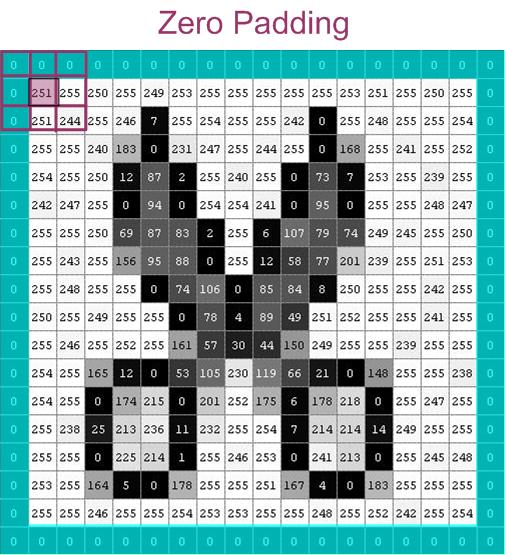
\includegraphics[width=0.33\linewidth]{Images/pad_zero_color.jpg}
	\caption{An image padded with zeroes. Convolution with the 3$\times$3 stencil will now preserve image size; but at what cost?}
\end{figure}



%%=================================================
%% Deconvolution
%%=================================================
\subsection{Full Image Deconvolution}

\subsubsection{Na\"ive ``First Look'}

In section~\ref{sec:kernel} we found the kernel $k$ which would transform a messy PSF image into a nice symmetrical one with known properties (\psfobs $\rightarrow$ \psfref.). This same kernel can be used to transform an entire image with the observed PSF, $\mathcal A$, into the same image with the target PSF, $\mathcal B$. To do this, we can perform the operation
\begin{align}
	\mathcal{B} &= k \ast \mathcal{A},
	\shortintertext{or, in the language of linear algebra,}
	\vec{b} &= \mathbf{K} \vec{a}.\label{eqn:simple_deconvolve}
\end{align}
The image vectors $\vec b$ and $\vec a$ have the same form as discussed earlier -- they are simply flattened versions of the pixel-arrays. The kernel matrix $\mathbf K$ is more tricky; but after some refelxion, it transpires that $\mathbf K$ is a sparse, upper-diagonal matrix where every row is identical, but shifted right by one element with respect to the row above. (Note that in practice it is unweildy and prohibitively expensive to store all the zero-entries of the $\mathbf K$ matrix -- we have to be a little bit clever about how to store and manipulate the relevant information.)

Once we have constructed an appropriate kernel matrix and multiplied it by the (observed) image vector, we are done.

Alternatively, we can simply use a pre-existing module which performs the convolution for us: \texttt{scipy.signal.fftconvolve} does the job nicely. We can even tell this module to reduce the size of the convolved image (\texttt{mode="valid"}), in keeping with the concerns raised in section~\ref{sec:shave} .

However, it would be naive to simply place our trust in SciPy -- their convolution method may be subtly different from the one we wish to use for scientific inference. Thus, we cannot escape having to implement the concolution procedure of equation~\ref{eqn:simple_deconvolve}. Figure~\ref{fig:deconvolution_comparison} shows a comparison, with residuals. Leaving aside the image arteficts from using a small convolution kernel (\MORE FIX!), we can see that the two methods do not agree completely. This is worrying, but according to DWH the problem is almost certainly with my implementation rather than SciPy's, and I am inclined to agree (it might be a simple indexing error). Combined with the fact that SciPy is around 15 times faster, it makes little sense to labour on with my code; so we adopt the SciPy convolution module.

\FIG{Comparison of my convolution algorithm with SciPy's.}

\begin{figure}
	\def\width{0.3\textwidth}
	\centering
	\begin{subfigure}{\width}
		\includegraphics[width=\textwidth]{../../Data/Deconvolved/gsc_CFHTLS_03_g_sci_rescaled.png}
		\caption{Original image}
	\end{subfigure}
	
	\begin{subfigure}{\width}
		\includegraphics[width=\textwidth]{../../Data/Deconvolved/gsc_CFHTLS_03_g_sci_rescaled_MAN.png}
		\caption{Deconvolved using my procedure and a 3x3 kernel.}
	\end{subfigure}
	~
	\begin{subfigure}{\width}
		\includegraphics[width=\textwidth]{../../Data/Deconvolved/gsc_CFHTLS_03_g_sci_rescaled_SCI.png}
		\caption{Deconvolved using SciPy's procedure and a 3x3 kernel.}
	\end{subfigure}
	
	\begin{subfigure}{\width}
		\includegraphics[width=\textwidth]{../../Data/Deconvolved/gsc_CFHTLS_03_g_sci_rescaled_RES.png}
		\caption{Residuals.}
	\end{subfigure}
	\caption{Deconvolution procedure -- a comparison of my home-made convolution algorithm and SciPy's optimised one. SciPy takes about 1/15 of the time. Note that a 3x3 kernel was used for this test, and there are obvious artifacts introduced around bright points of the image.}
	\label{fig:deconvolution_comparison}
\end{figure}

So why does the heading for this subsection include the word ``na\"ive''? Have we done something wrong?
\begin{itemize}
	\item Over-constrained -- solution could be messy
	\item Want to smooth solution
\end{itemize}


\subsubsection{A Better Method}

Here we adopt the more robust and powerful method due to \citet{MCS98}. Instead of finding the deconvolved image, $\mathcal A$, by minimising the residuals for equation~\ref{eqn:simple_deconvolve}, we split the final image into its point sources -- amplitude-$\alpha$ $\delta$-functions at (2D) position $c$ --, and a smooth background, $h$; then we minimise the functional $S\left[\{\alpha\},\{c\}, h \,\middle|\, {d}, {\sigma}, {r}, {k}, \lambda \right]$ with respect to its left-hand arguments:
\begin{align}
	S = \sum_{i=1}^N \frac{1}{\sigma_i^2} \left[ \sum_{j=1}^N k_{ij} \left(h_j +\sum_{k=1}^M \alpha_k r(x_j-c_k)\right) - d_i \right]^2\
			+\; \lambda\sum_{i=1}^N \left( h_i - \sum_{j=1}^N r_{ij}h_j \right)^2 \label{eqn:minimisation_functional}
\end{align}
(equation~(7) of their paper). This requires some explanation. First, what do all the symbols denote?\footnote{Note that in the argument of $S$ above, we've dropped the vector/matrix notations. Indeed, the form of the variables is somewhat elastic, depending on how we choose to set up the problem. So although it might be tempting at first glance to assume the single-index variables of equation~\ref{eqn:minimisation_functional} are like vectors and the double-index variables are like matrices, we actually have some freedom in how to express them. For instance, the ``vector'' $d_i$ represents the original \emph{2D} image. So in order to understand what's going on in the equation, we should keep in mind the \emph{number} of independent elements each object has.} This is listed in table~\ref{tbl:minimisation_functional}.

\begin{center}
	\begin{table}[h!]
		\begin{tabularx}{\textwidth}{l | X | X}
			\hline
			Variable	& Description & Role\\ \hline
			%
			$S$ 	& A functional & For minimisation\\ \hline
			%
			$\sigma_i$ & Standard deviation of the image at pixel $i$. Has $N$ elements. & Calculated from the data.\\ \hline
			%
			$k_{ij}$	& Deconvolution kernel. Has a user-specified number of elements. & Calculated here from PSFEx\ldots\\ \hline
			%
			$h_j$		& The pixels of the ``true'' image or scene which describe everything except the point sources. $N$ elements. & This is an object to be found via the minimisation procedure. Requires an intial guess, $h^0$.\\ \hline
			%
			$\alpha_k$	& Enodes the intenitisties of the image's point sources. Number of elements, $M$ obviously depends on the image. & This is an object to be found via the minimisation procedure. Requires an intial guess, $a^0$.\\ \hline
			%
			$c_k$	& Enodes the positions of the image's point sources. Since each source has two coordinates, $c$ has $2M$ elements. & This is an object to be found via the minimisation procedure. Requires an intial guess, $c^0$.\\ \hline
			%
			$r(x_j)$	& The target PSF. Size is set by user. & From PSFEx\ldots\\ \hline 
			%
			$d_i$	& Original image, or data. & What we start with.\\ \hline
			%
			$\lambda$	& A lagrange multiplier. & Set by the user to ensure the deconvolved image has the right statistical properties.\\
			%
			\hline
		\end{tabularx}
		\caption{Listing the variables in equation~\ref{eqn:minimisation_functional}, from left to right.}
		\label{tbl:minimisation_functional}
	\end{table}
\end{center}

Now we know what all the symbols mean, we can begin to see some structures.
\begin{equation}
	\left(h_j +\sum_{k=1}^M \alpha_k r(x_j-c_k)\right)
\end{equation}
is simply our reconstructed image, with background and point sources, while
\begin{equation}
	s_{ij}\left(h_j +\sum_{k=1}^M \alpha_k r(x_j-c_k)\right)
\end{equation}
``re-blurs'' the reconstruction for comparison with the data, $d_i$. The first term of equation~\ref{eqn:minimisation_functional} is therefore a $\chi^2$ term for our model and our data, albeit with the model decomposed into two pieces.

The second term is included to ensure smoothness of the background\ldots \MORE

We can re-express the minimisational functional in terms of a linear algebra operation. The most immediate way is
\begin{align}
	S = \left\{ \frac{1}{\vec\sigma} \left[ \mathbf k \left( \vec{h} + \vec{\alpha^\prime} \ast r \right) - \vec{d} \right]\right\}^2\
			+\; \lambda \left( \vec{h} - \mathbf{r}\vec{h} \right)^2, \label{eqn:minimisation_functional_linalg}
\end{align}
where, to be totally explicit, we've listed all the variables again in table~\ref{tbl:minimisation_functional_linalg}.

\begin{center}
	\begin{table}[h!]
		\begin{tabularx}{\textwidth}{l | X | X}
			\hline
			Variable	& Description & Comments\\ \hline
			%
			$S$ 	& A functional & For minimisation\\ \hline
			%
			$\vec\sigma$ & Standard deviation of image at each pixel. A vector of length $N$. & Calculated from the data.\\ \hline
			%
			$\mathbf k$	& Deconvolution kernel. Has a user-specified number of independent elements, but is here represented by an $N\!\times\!N$ matrix. & Calculated from PSFEx\ldots\\ \hline
			%
			$\vec h$		& The pixels of the ``true'' image or scene which describe everything except the point sources. Vector of length $N$. & This is an object to be found via the minimisation procedure. Requires an intial guess, $\vec h^0$.\\ \hline
			%
			$\vec{\alpha^\prime}$	& Enodes the intenitisties of the image's point sources. Number of elements, $M$ obviously depends on the image. & This is an object to be found via the minimisation procedure. Requires an intial guess, $\vec{\alpha^\prime}^0$.\\ \hline
			%
			$r$	& The target PSF. Size is set by user. & From PSFEx\ldots\\ \hline 
			%
			$\vec d$	& Original image, or data. $N$-element vector. & What we start with.\\ \hline
			%
			$\lambda$	& A lagrange multiplier. & Set by the user to ensure the deconvolved image has the right statistical properties.\\
			%
			\hline
		\end{tabularx}
		\caption{Listing the variables in equation~\ref{eqn:minimisation_functional_linalg}, from left to right.}
		\label{tbl:minimisation_functional_linalg}
	\end{table}
\end{center}

We can still readily see the structure of what's going on. \MORE

%%=================================================
%% Test Noise Properties
%%=================================================
\subsection{Noise Properties}

Here I've applied a few different stretches to the original image and to the deconvolved image. The left-hand side images are all stretched originals and the right-hand side are all stretched deconvolutions. The stertch gets more sever as you go down.


Specific notes:\\
* I used a 9x9 kernel for these images.\\
* To change the strength of the stretch, I simply divided the upper bound (you called it "vmax") by 2 and 10.\\

\includepdf[pages={1,2}]{../../Data/Deconvolved/CFHTLS_03_g_Deconvolved_noisecompare.pdf}


%%=================================================
%% Image Manipulation
%%=================================================
\subsection{Image Manipulations}

\begin{itemize}
	\item Making them viewable by humans -- stretch
	\item .psf file conversion
	\item FITS conversion
\end{itemize}




%%=================================================
%% RBG
%%=================================================
\section{Colour Combination}
\label{sec:colour}

Telescope data is often given in ``bands'' -- we do not record the total flux coming from a point in the sky, but the flux in a certain wavelength range. This information allows us to investigate the properties of astronomical objects, such as temperature and chemical composition. However to make a readily-interprable image which contains maximum information in one hit, we need to combine the bands to make a colour-composite image.

Many methods had been developed to do this in accordance with researchers' individual aesthetic preference. But the full richness of possibility was still unexploited, until \citet{Lup++04} demonstrated just how much detail one could extract from data when colour was given its deserved treatment (see appendix~\ref{sec:Lup++04notes} for more detail). Using their method, we can combine images from different bands in a way which enhances hidden or faint features without allowing bright objects to dominate. It has the further advantage that the brightness of an object in the image is decoupled from its colour. The method is implemented in PJM's \emph{HumVI} (formerly \emph{ColorJPG}).

A further improvement to the method was implemented by Wherry (\MORE describe difference
\footnote{PHIL: `My reading of it is that Lupton uses two parameters, Q and alpha, to
tweak the look of the image, while Wherry's IDL code takes 4 input
parameters: 3 image scales and a nonlinearity parameter.
I like Wherry's approach because I *think* I want to make images that
all have the same scales and limits, that is, that a pixel of a
particular colour and brightness in field1.png is representing the
same set of surface brightnesses that a pixel of equal colour and
brightness is in field2.png. I want to develop intuition about the
objects, and the noise level, through displaying a lot of images! Note
that display of noise is itself an issue - I am unlikely to want to
use your "kill noise" option, but am happy for the zero surface
brightness level in the image to be dark grey instead of black.

Anupreeta More has made a very nice set of test CFHTLS images for the
Lens Zoo, and I discussed with her a bit your work: she thinks we
should do a blind taste test at some point, showing the lens zoo dev
team her images that have been a) displayed in standard form with
HumVI and b) deconvolved and then
displayed in standard form with HumVI, and ask for them to be graded
for arc visibility. Probably we would want to supply a few different
standard forms as well (and by "form" I mean {scales,nlin}). We can
also do image testing at Adler Planetarium on the willing public
there. The question we want to answer is: "how should we display an
image to maximize the likelihood of an untrained human seeing
interesting feature X?"  I have no idea where one sends paper like
this - Ill ask the zooniverse team.'}
). We translated Wherry's improvements from IDL to Python, and integrated this module with the HumVI code. Some additional improvements are also made, such as increased versatility with rebinning.

A summary of this part of the project (with pseudocode) follows.

\begin{enumerate}
	\item Translated (and improved?) the Wherry algorithm from IDL to Python (\texttt{wherry.py}). This is what it does:
	\texttt{
	\begin{enumerate}
		\item RGB = [readin(R\_data),readin(G\_data),readin(B\_data)]		\#\# *\_data can be filename, array of data, or a channel instance
		\item rescale(RGB, scalefactors)	\#\# multiply each band by a given number
		\item rebin(RGB, xrebinfactor,yrebinfactor)		\#\# re-sample images
		\item kill\_noise(RGB, cutoff)	\#\# sets all pixels below a threshold to 0
		\item arsinh\_stretch(RGB, nonlinearity)
		\begin{itemize}
			\item pixtot = R\_array+G\_array+B\_array	\#\# collapse images onto each other
			\item if pixtot[i,j]==0: pixtot[i,j]=1
			\item factor = arsinh(nonlin*rad)/(nonlin*rad)
			\item (R\_array,G\_array,B\_array) *= factor
		\end{itemize}
		\item if stauratetowhite==False: box\_scale(RGB)
		\begin{itemize}
			\item maxpixel[i,j] = max(R[i,j],G[i,j],B[i,j])	\#\# i.e. find the maximum pixel value of the three arrays
			\item if maxpixel[i,j] < 1: maxpixel[i,j]=1
			\item (R\_array,G\_array,B\_array) /= maxpixel
			\item (Also translates origin of image if required)
		\end{itemize}
		\item overlay/underlay \#\# not entirely sure what these are for
		\item scipy.misc.imsave(RGB)
	\end{enumerate}
	}
	\begin{itemize}
		\item Note: when treating \texttt{wherry.py} as a standalone code for making composite images, the user can choose which bands to use for R, G and B.
		\item Also, in the IDL version of the code, there is a function devoted to transforming the image data into bytes. When I was translating to Python, I found that this was an unnecessary IDL-specific step, and it was unnecessary to implement it.
	\end{itemize}
	\item Integrated with PJM's HumVI code, so that choice of Lupton/Wherry procedure is an option.
	\begin{itemize}
		\item Wherry is default. Luption can be invoked with command-line keyword \texttt{--lupton} or simply \texttt{-l}.
		\item Again, the user can choose which bands to use for R, G and B -- it just depends on the order of the three filenames.
		\begin{itemize}
			\item After some initial misunderstanding, I now use R=i, G=r, B=g.
		\end{itemize}
		\item Of course, this bands$\rightarrow$colour map is unchanged when when \texttt{--lupton} is specified.
	\end{itemize}
\end{enumerate}

%\begin{figure}
%  \centering
%    %\includegraphics[width=\linewidth]{C:/Users/adam.BEYOND/Dropbox/Hogg_2012/Code/HumVI/images/test/CFHTLS_03_lw.pdf}
%  \caption{Restretched images and combination of three bands using two different procedures. \MORE specifics of algorithm / equation / pseudocode. \MORE crop.}
%\end{figure}




%%=================================================
%% UNMBRELLA
%%=================================================
\section{Combined Deconvolution and Colour}
\ref{sec:combine}

\citet{MCS98} -- must deconvolve all bands to target PSF before combining.


\newpage
%%=================================================
%% TO DO
%%=================================================
\section{To do}

\underline{Document}
\begin{itemize}
	\item Invert figure colours to save ink\newline
	[Latex can't do this, I'll have to make them myself.]
\end{itemize}

\underline{Colour}
\begin{itemize}
	\item Make some side-by-side composites showing Wherry and Lupton
	\item Fail to compute scales $\rightarrow$ error
	\item Should work with one or two FITS images.
\end{itemize}

\underline{Deconvolution}
\begin{itemize}
	\item How does kernel size affect execution time?
	\item Invent quality metrics: each one represents the quantitiave answer to a particular question about some aspect of the reconstructed image -- its "noise" level, the correlated nature of that noise, the number of false SExtractor detections (in the reconstructed image) generated, the SExtractor flux of certain
objects of interest, the number of inspectors who identify feature X, etc etc etc. We can propose and discuss these aspects after seeing some images.
	\item arcsec\ra pixels method; will need header information.
	\item Assert target PSFs of width 0.3,0.4,0.5,0.6,0.7,0.8,0.9, 1.0 arcsec FWHM, and make deconvolved images for each value. Then plot your quality metric(s) against FWHM.
	\item Homogenise PSF across different fields. \TODO{What is the best way to do this?} Use largest PSF $\rightarrow$ no danger of violating sampling theorem; but this may be way too blurry to be useful. Pickle.
\end{itemize}

\underline{Combining C\&D}
\begin{itemize}
	\item Determine some metrics for successful combination / sensitivity to interesting features. Modify stretch / \psfref appropriately.
\end{itemize}

\underline{Maths}
\begin{itemize}
	\item PHIL: `I would like to see a derivation of this procedure, which involves a
matrix acting on a noisy vector. Do you start by writing down the
principled probabilistic inference of a model image given noisy data,
and end up showing that this boils down (under certain assumptions) to
the matrix operations you perform? Any improvements we make to your
code will probably be of the form "assign a different prior to the
pixel values of the kernel/final image", so it'd be good to see how
that propagates through into new matrix operations.'

	\item A prior on pixel values would lead to an
additional term (with a lagrange multiplier) added to the summed
squared residuals. It would be good to also include the weight image, that
characterises the actual per pixel uncertainty, because some pixels
are going to have very high uncertainty indeed... We need to be able
to cope with saturated pixels, chip gaps etc, and weight images is how
you do it, in general.
\end{itemize}




\newpage
%%=================================================
%% APPENDIX
%%=================================================
\appendix
\addcontentsline{toc}{section}{Appendix}
\section*{APPENDIX}

%%=================================================
%% MCS 1998 paper
%%=================================================
\section{\citet{MCS98} -- ``Deconvolution with Correct Sampling''}
\label{sec:MCS98notes}

\paragraph{Key Ideas}

-- We shouldn't pretend to derive infinite resolution images from discrete data. A more honest approach can mitigate the appearance of 
artefacts.

-- Bear in mind that correlations in astrnomical images are local. Global treatments and techniques are inappropriate.


\paragraph{Background}

-- Ground-based telescopes suffer from aperture diffraction and from atmospheric inhomogeneities which distort light. One (post hoc) way of 
correcting for this is to infer the point spread function from a puative point source in your image; if we consider the data to represent 
"reality" or the "scene" convolved with this PSF, then we can in principle deconvolve the data from the PSF to retrieve the scene. 

-- There will be many scenes compatible with the (uncertain) data, so we must then pose the problem as an optimisation problem: we wish to 
find the scene, compatible with the data, that minimises some cost function to be devised. A typical procedure is to minimise the chi-squared 
function (between data and model).

-- Also want solution to be smooth, so introduce a Lagrange function which enforces this. A common procedure is to maximise the entropy of the 
image (using the flux distribution as the information). This has the benefit of requiring positive flux values.

-- So far we ignore noise in the image.

\paragraph{Problems}

-- Two problems emerge with this way of doing things: 1) often find image artefacts (from improper sampling, as we shall see); 2) it doesn't 
preserve the global intensity scale.

-- In practice, telescope cameras are constructed so that their data just satisfy the sampling theorem -- the pixel-spacing is ~2x the maximum 
frequency expected from objects. Upon deconvolution, where the fuzziness is taken out, the sampling theorem will be violated. Theoretically, 
deconvolution can introduce point-sources/Dirac-deltas (i.e. stars), so an infinitely small sampling interval would have to be used.

-- Deconvolution therefore leads to artefacts when there is a sharp discontinuity in the scene -- e.g. a star on a black background shows 
ringing. (Can think of this as a window in frequency space (i.e. a cutoff at some maximum frequency) leading to a sinc function in position-
space: the result of deconvolving a point source will be delta*sinc.)

-- In traditional methods, riniging is mitigated by the positivity 
constraint, which damps down the lobes of oscillations. But this depends crucially on the zero-level, and accurate subtraction of sky noise 
is necessary for the methods to wrok well.

-- Image artefacts steal flux and bias photometry. Also, maximising entropy makes the image as 
smooth (uniform) as possible, which tends to spread out point sources; peak intensity is thus undersetimated.


\paragraph{Proposal}

-- Do not do a full deconvolution: do a "light" deconvolution where point sources are given as extended objects of know size and flux 
distribution. These objects are chosen such that they satisfy the sampling theorems. In other words, reconstruct the image you would get if 
you had a better instrument (rather than a perfect instrument).

-- So now the image has a constant PSF, which MCS call r(x). This introduces a length scale over which the image must be smooth (?). This 
applies to point sources (which have shape r(x)) and extended sources. From the solution space of lightly-deconvolved scenes, we should 
choose the one which gives maximum smoothness on this local scale.

-- Specifically, for each pixel we take the difference of the "background" (everything which isn't delta) from the "reconstrcuted background" 
(the fixed PSF convolved with the scene); then sum over pixels and minimise (equation 7). This procedure discards high-frequency information, 
but is consistent with the adopted sampling and the frequencies of r(x).

-- Artefacts not stealing flux AND no smoothing of point sources -> 
photometry possible.

-- Requires no positivity constraint.


\paragraph{Usage}

-- Using simulated and real astronomical images, with finite resolution and noise, the new procedure is compared with other standard 
procedures and does (stupidly) well. They are able to recover fluxes and positions to high accuracy, and they avoid exacerbating noise / 
artefacts in the image.

-- Image combination is also demonstrated -- deconvolution of many images to the same PSF before combining them yields 
high-resolution final image.


\paragraph{Further Work}

-- Devise a more robust optimisation that finds minimum even in populated images.


%%=================================================
%% Lupton & al. 2004 paper
%%=================================================
\section{\citet{Lup++04} -- ``Preparing Red-Green-Blue Images from CCD Data''}
\label{sec:Lup++04notes}

\paragraph{Quote}

'sheer drama and beauty of the night sky'

\paragraph{Key Idea}

-- There is a lot of information in the colouration of an image. This often helps us distinguish features / phenomena and classify astronomical objects.

-- Hitherto, focus has been on {\it intensity} differences.


\paragraph{Background}

-- We apply stretches to images in order to coax faint objects into observability. But we must strike a balance between this objective and the saturation of bright parts.

-- Stretch is a re-scale, bringing all objects to within a brightness cutoff range. Re-scale can be linear, ln, sqrt, depending on preference and the diversity of images.

-- Tuning parameters is not always straightforward. Any object above maximum brightness ends up bleached and obese.

-- Furthermore, there is degeneracy between brightness and colour in traditional stretching procedures.


\paragraph{Solution}

-- Using a different stretching procedure, (equation 2), can discard uninteresting intensity information in favour of colour information. This works by comparing the individual colour-intensities to the total intensity (i.e. ~ compare the colours amongst themselves), and comparing the total instensity to the two cutoff intensities which define the brightness scale.

-- NB the colours are unique -- no degeneracy with intensity. So we can draw unambigouous conclusions from looking at colour differences.

-- arsinh stretch magnifies faint objects (linear regime) and avoids bleaching bright objects (logarithmic regime). (But this could be achieved with other functions too).


\paragraph{Examples}

-- Some examples are given where the standard technique loses an embarrassing amount of detail compared with the new idea. By eye, we clearly distinguish differences between objects which are otherwise just rendered as white blobs.


\newpage
\addcontentsline{toc}{section}{References}
\bibliographystyle{plainnat}
\bibliography{humvi}

\end{document}
